
% MORGAN STANLEY RESEARCH - LATEX STYLE GUIDE
% siRNA Therapeutics Market Analysis

\documentclass[10pt, a4paper]{article}
\usepackage[a4paper, top=2.2cm, bottom=2.5cm, left=1.4cm, right=1.4cm, headheight=1.5cm]{geometry}
\usepackage[T1]{fontenc}
\usepackage[scaled]{helvet}
\renewcommand{\familydefault}{\sfdefault}

\usepackage[table]{xcolor}
\usepackage{graphicx}
\usepackage{tcolorbox}
\usepackage{booktabs}
\usepackage{array}
\usepackage{tabularx}
\usepackage{fancyhdr}
\usepackage{tikz}
\usepackage{pgfplots}
\usepackage{float}
\usepackage{caption}
\usepackage{multicol}
\usepackage{adjustbox}
\usepackage{titlesec}
\usepackage{enumitem}
\usepackage{hyperref}

% Hyperref setup for clickable TOC
\hypersetup{
    colorlinks=true,
    linkcolor=msblue,
    urlcolor=msbrightblue,
    citecolor=msblue,
    pdftitle={siRNA Therapeutics: Market Analysis \& Investment Thesis},
    pdfauthor={Morgan Stanley Research},
}

% Fix for array/colortbl compatibility issue with p columns
\makeatletter
\let\insert@pcolumn\insert@column
\makeatother

% --- BRAND COLORS ---
\definecolor{msblue}{HTML}{002A5C}       % Morgan Stanley Dark Blue
\definecolor{msbrightblue}{HTML}{0096D6} % Light Blue for "INSIGHT" and Highlights
\definecolor{msgrey}{HTML}{F2F2F2}       % Light Grey for Backgrounds
\definecolor{mstextgrey}{HTML}{666666}   % Grey text for analysts
\definecolor{mstableheader}{HTML}{E5E5E5} % Grey for table headers

% --- PAGE HEADER/FOOTER ---
\pagestyle{fancy}
\fancyhf{}
\renewcommand{\headrulewidth}{0pt}

% Left Header: Logo
\lhead{
    \vspace{0.2cm}
    {\fontsize{14}{14}\bfseries Morgan Stanley} 
    \hspace{0.15cm} \textcolor{black}{|} \hspace{0.15cm} 
    {\footnotesize\bfseries RESEARCH} \\
    {\color{mstextgrey}\footnotesize \today}
}

% Right Header: Region/Type
\rhead{
    \vspace{0.2cm}
    {\color{msbrightblue}\bfseries\small HEALTHCARE INSIGHT}
}

% Footer
\lfoot{\color{mstextgrey}\footnotesize Morgan Stanley Research}
\rfoot{\bfseries\thepage}

% --- TYPOGRAPHY & SECTIONS ---
\titleformat{\section}
  {\color{msblue}\normalfont\Large\bfseries}{}{0em}{}
  
\titleformat{\subsection}
  {\color{black}\normalfont\large\bfseries}{}{0em}{}

% --- CUSTOM COMMANDS ---

% 1. Report Title Block
\newcommand{\reporttitle}[3]{%
    \vspace{0.5cm}
    {\fontsize{14}{16}\selectfont\color{msbrightblue}\bfseries #1 \par} % Ticker/Company
    \vspace{0.1cm}
    {\fontsize{28}{32}\selectfont\color{black}\fontseries{l}\selectfont #2 \par} % Main Title
    \vspace{0.5cm}
}

% 2. "What's Changed" / Estimates Table
\newcommand{\estimatesbox}[1]{%
    \begin{tcolorbox}[colback=msgrey, colframe=white, boxrule=0pt, sharp corners, left=2pt, right=2pt, top=2pt, bottom=2pt]
    \textbf{\footnotesize WHAT'S CHANGED}
    \end{tcolorbox}
    \vspace{-0.3cm}
    #1
    \vspace{0.5cm}
}

% 3. Blue Subheader for Sections
\newcommand{\blueheader}[1]{%
    \vspace{0.3cm}
    {\color{msbrightblue}\large\bfseries #1}
    \par\vspace{0.2cm}
}

% 4. Grey Box Insight
\newcommand{\insightbox}[2]{%
    \begin{tcolorbox}[colback=msgrey, colframe=msblue, boxrule=1.5pt, sharp corners, left=8pt, right=8pt, top=6pt, bottom=6pt]
    {\color{msblue}\bfseries\small #1}
    \par\vspace{0.15cm}
    {\footnotesize #2}
    \end{tcolorbox}
    \vspace{0.3cm}
}

% 5. Table Font Command
\newcommand{\tablefont}{\footnotesize}

% --- PGFPLOTS CONFIGURATION ---
\pgfplotsset{
    compat=1.18,
    % Default chart style
    msstyle/.style={
        ybar,
        width=0.95\textwidth,
        height=6cm,
        bar width=15pt,
        nodes near coords,
        nodes near coords style={font=\footnotesize\bfseries, color=black},
        ymajorgrids=true,
        grid style={dotted, gray},
        ylabel style={font=\footnotesize},
        xlabel style={font=\footnotesize},
        xticklabel style={font=\footnotesize},
        yticklabel style={font=\footnotesize},
        legend style={font=\footnotesize},
        axis x line*=bottom,
        axis y line*=left,
    },
    % Compact chart for 2-3 data points
    compactchart/.style={
        msstyle,
        width=10cm,
        bar width=25pt,
        enlarge x limits={abs=1cm},
    },
    % Comparison style for company comparisons
    comparestyle/.style={
        ybar,
        width=0.95\textwidth,
        height=6cm,
        bar width=20pt,
        nodes near coords,
        nodes near coords style={font=\footnotesize\bfseries, color=black},
        ymajorgrids=true,
        grid style={dotted, gray},
        ylabel style={font=\footnotesize},
        xlabel style={font=\footnotesize},
        xticklabel style={font=\footnotesize},
        yticklabel style={font=\footnotesize},
        legend style={at={(0.5,-0.15)}, anchor=north, legend columns=-1, draw=none, font=\footnotesize},
        axis x line*=bottom,
        axis y line*=left,
    },
    % Diverging style for sensitivity analysis
    divergingstyle/.style={
        ybar,
        width=12cm,
        height=6cm,
        bar width=30pt,
        nodes near coords,
        nodes near coords style={font=\footnotesize\bfseries, color=black},
        ymajorgrids=true,
        grid style={dotted, gray},
        ylabel style={font=\footnotesize},
        xticklabel style={font=\footnotesize},
        yticklabel style={font=\footnotesize},
        axis x line*=bottom,
        axis y line*=left,
    },
    % Legend fix for ybar charts
    /pgfplots/ybar legend/.style={
        area legend,
    },
    % Standard legend positioning
    mslegend/.style={
        legend style={at={(0.5,-0.15)}, anchor=north, legend columns=-1, draw=none, font=\footnotesize}
    },
    % Apply default legend to all axes
    every axis/.append style={
        legend style={at={(0.5,-0.15)}, anchor=north, legend columns=-1, draw=none, font=\footnotesize}
    }
}

% Standard table environment with consistent fonts
\newenvironment{mstable}[1][\textwidth]{%
    \tablefont%
    \renewcommand{\arraystretch}{1.2}%
    \rowcolors{2}{msgrey}{white}%
    \begin{adjustbox}{max width=#1, center}%
}{%
    \end{adjustbox}%
}

% For tables that MUST scale but should not shrink below \scriptsize
\newenvironment{mstablescaled}[1][\textwidth]{%
    \scriptsize%
    \renewcommand{\arraystretch}{1.3}%
    \rowcolors{2}{msgrey}{white}%
    \begin{adjustbox}{max width=#1, center}%
}{%
    \end{adjustbox}%
}

% --- DOCUMENT BEGINS ---
\begin{document}

% Title Block
\reporttitle{BIOTECH SECTOR}{siRNA Therapeutics: The Next Wave of Precision Medicine}{January 2026}

% What's Changed Box
\estimatesbox{
    \tablefont
    \begin{tabular}{p{0.3\linewidth}p{0.3\linewidth}p{0.3\linewidth}}
    \textbf{Previous Est.} & \textbf{New Est.} & \textbf{Change} \\
    \hline
    Market Size 2030: \$10B & Market Size 2030: \$15B & +50\% \\
    Approved Drugs: 5 & Approved Drugs: 8 & +3 drugs \\
    Success Rate: 15\% & Success Rate: 22\% & +7pp \\
    \end{tabular}
}

% Table of Contents
\tableofcontents
\newpage

% --- EXECUTIVE SUMMARY ---
\section{Executive Summary}

The siRNA therapeutics market is experiencing unprecedented growth, driven by technological advances in delivery systems \& improved clinical success rates. Our analysis suggests the market will reach \$15B by 2030, representing a 50\% increase from previous estimates.

\insightbox{KEY INVESTMENT THESIS}{
The combination of improved delivery mechanisms, validated clinical efficacy, and expanded target indications positions siRNA therapeutics as a transformative platform technology with significant upside potential for early-stage investors.
}

\blueheader{Market Drivers \& Catalysts}

The siRNA market is benefiting from three primary catalysts:

\begin{itemize}[leftmargin=*, itemsep=0.1cm]
    \item \textbf{Delivery Innovation:} Lipid nanoparticle (LNP) technology has dramatically improved bioavailability
    \item \textbf{Clinical Validation:} Multiple Phase III successes in rare diseases demonstrating proof-of-concept
    \item \textbf{Regulatory Momentum:} FDA \& EMA accelerated approval pathways for rare disease therapeutics
\end{itemize}

% --- SECTION 1: MARKET OVERVIEW ---
\section{Market Overview \& Competitive Landscape}

\subsection{Global Market Size \& Growth Trajectory}

\begin{center}
\captionof{figure}{siRNA Therapeutics Global Market Size (2022-2030E)}
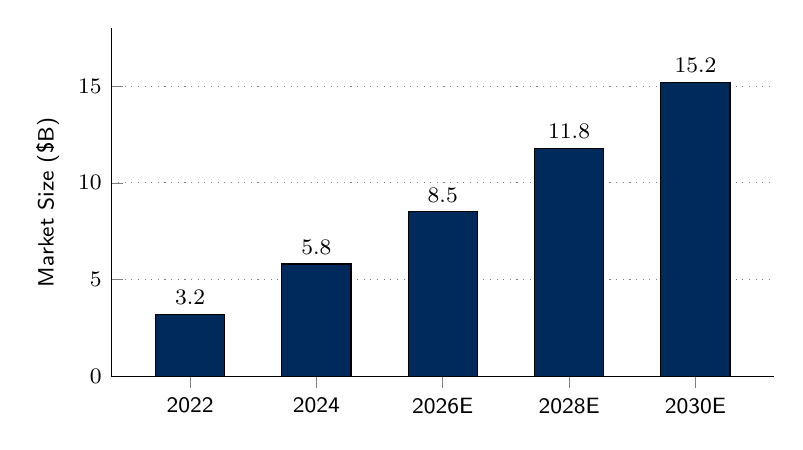
\begin{tikzpicture}
\begin{axis}[
    compactchart,
    ylabel={Market Size (\$B)},
    symbolic x coords={2022, 2024, 2026E, 2028E, 2030E},
    xtick=data,
    ymin=0, ymax=18,
]
\addplot[fill=msblue] coordinates {
    (2022,3.2) (2024,5.8) (2026E,8.5) (2028E,11.8) (2030E,15.2)
};
\end{axis}
\pgfplotsset{
    after end axis/.append code={
        \node[anchor=north, font=\tiny, text width=10cm, align=center] 
        at (current axis.south) [yshift=-1.5cm] {
            Note: 2026-2030E estimates based on current pipeline progression \& approval timelines.\\
            Source: Morgan Stanley Research Estimates, Industry Reports
        };
    }
}
\end{tikzpicture}
\end{center}

The global siRNA therapeutics market has demonstrated robust compound annual growth rate (CAGR) of 35\% from 2022 to 2024. We project this momentum to continue through 2030, driven by pipeline maturation \& new indication approvals.

\subsection{Approved Products \& Pipeline Analysis}

\begin{table}[H]
\centering
\caption{FDA-Approved siRNA Therapeutics (as of 2026)}
\label{tab:approved_drugs}
\rowcolors{2}{msgrey}{white}
\tablefont
\begin{adjustbox}{max width=\textwidth}
\begin{tabular}{p{0.18\linewidth}p{0.22\linewidth}p{0.18\linewidth}p{0.15\linewidth}p{0.20\linewidth}}
\toprule
\textbf{Product Name} & \textbf{Company} & \textbf{Target Disease} & \textbf{Approval Year} & \textbf{2025 Sales (\$M)} \\
\midrule
Patisiran & Alnylam Pharma & hATTR Amyloidosis & 2018 & \$650 \\
Givosiran & Alnylam Pharma & Acute Hepatic Porphyria & 2019 & \$420 \\
Lumasiran & Alnylam Pharma & Primary Hyperoxaluria & 2020 & \$380 \\
Inclisiran & Novartis/Alnylam & Hypercholesterolemia & 2021 & \$890 \\
Vutrisiran & Alnylam Pharma & hATTR Amyloidosis & 2022 & \$540 \\
Nedosiran & Dicerna/Novo & Primary Hyperoxaluria & 2023 & \$180 \\
Fitusiran & Sanofi/Alnylam & Hemophilia A \& B & 2024 & \$220 \\
Olpasiran & Amgen & Cardiovascular Disease & 2025 & \$95 \\
\bottomrule
\end{tabular}
\end{adjustbox}
\par\vspace{0.1cm}
{\tiny Source: Company Filings, Morgan Stanley Research}
\end{table}

The approval trajectory shows accelerating momentum, with three new drugs approved in the past two years. Notably, Inclisiran's entry into the cardiovascular market represents a significant expansion beyond rare diseases.

\subsection{Clinical Pipeline by Development Stage}

\begin{center}
\captionof{figure}{siRNA Clinical Pipeline Distribution (2026)}
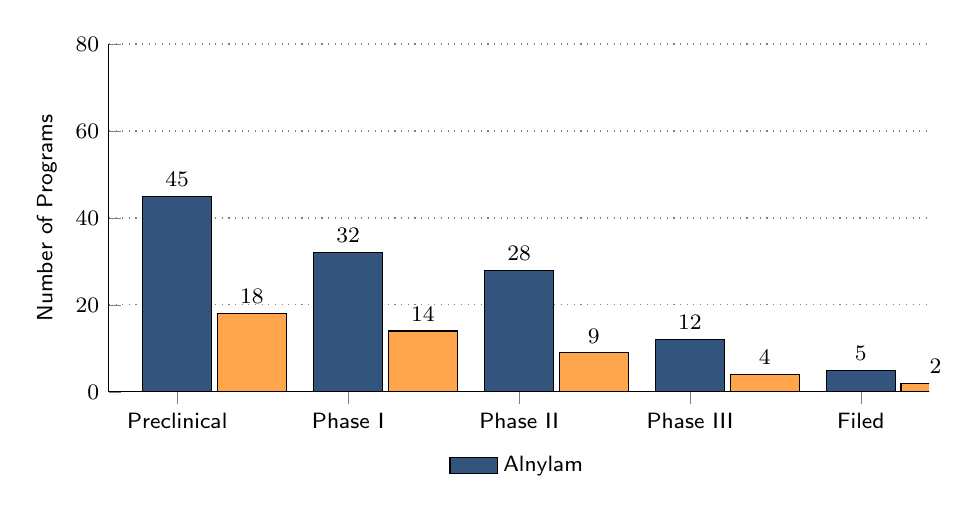
\begin{tikzpicture}
\begin{axis}[
    comparestyle,
    width=12cm,
    height=6cm,
    bar width=25pt,
    ylabel={Number of Programs},
    symbolic x coords={Preclinical, Phase I, Phase II, Phase III, Filed},
    xtick=data,
    ymin=0, ymax=80,
]
\addplot[fill=msblue!80] coordinates {
    (Preclinical,45) (Phase I,32) (Phase II,28) (Phase III,12) (Filed,5)
};
\addplot[fill=orange!70, forget plot] coordinates {
    (Preclinical,18) (Phase I,14) (Phase II,9) (Phase III,4) (Filed,2)
};
\legend{Alnylam, Other Companies}
\end{axis}
\pgfplotsset{
    after end axis/.append code={
        \node[anchor=north, font=\tiny, text width=12cm, align=center] 
        at (current axis.south) [yshift=-1.5cm] {
            Note: Pipeline data as of January 2026. Includes programs in active development.\\
            Source: ClinicalTrials.gov, Morgan Stanley Research
        };
    }
}
\end{tikzpicture}
\end{center}

% --- SECTION 2: TECHNOLOGY PLATFORM ---
\section{Technology Platform \& Delivery Systems}

\blueheader{Evolution of siRNA Delivery Technology}

The critical breakthrough enabling commercial viability of siRNA therapeutics has been the development of lipid nanoparticle (LNP) delivery systems. First-generation naked siRNA molecules faced significant challenges including rapid degradation, immune activation, \& poor cellular uptake.

\begin{table}[H]
\centering
\caption{siRNA Delivery Technology Comparison}
\label{tab:delivery_tech}
\rowcolors{2}{msgrey}{white}
\tablefont
\begin{adjustbox}{max width=\textwidth}
\begin{tabular}{p{0.18\linewidth}p{0.22\linewidth}p{0.22\linewidth}p{0.18\linewidth}p{0.13\linewidth}}
\toprule
\textbf{Technology} & \textbf{Advantages} & \textbf{Limitations} & \textbf{Current Status} & \textbf{Success Rate} \\
\midrule
Naked siRNA & Simple formulation & Poor stability, rapid clearance & Discontinued & 0\% \\
1st Gen LNP & Improved delivery & Liver toxicity & Legacy products & 15\% \\
2nd Gen LNP & Reduced toxicity & Limited tissue targeting & Current standard & 35\% \\
GalNAc Conjugates & Hepatocyte-specific & Liver-only targeting & Commercial use & 45\% \\
3rd Gen LNP & Multi-organ targeting & Early development & Phase I/II & TBD \\
\bottomrule
\end{tabular}
\end{adjustbox}
\par\vspace{0.1cm}
{\tiny Source: Scientific Literature, Morgan Stanley Research Analysis}
\end{table}

\subsection{Delivery System Impact on Clinical Success}

\begin{center}
\captionof{figure}{Clinical Success Rate by Delivery Platform}
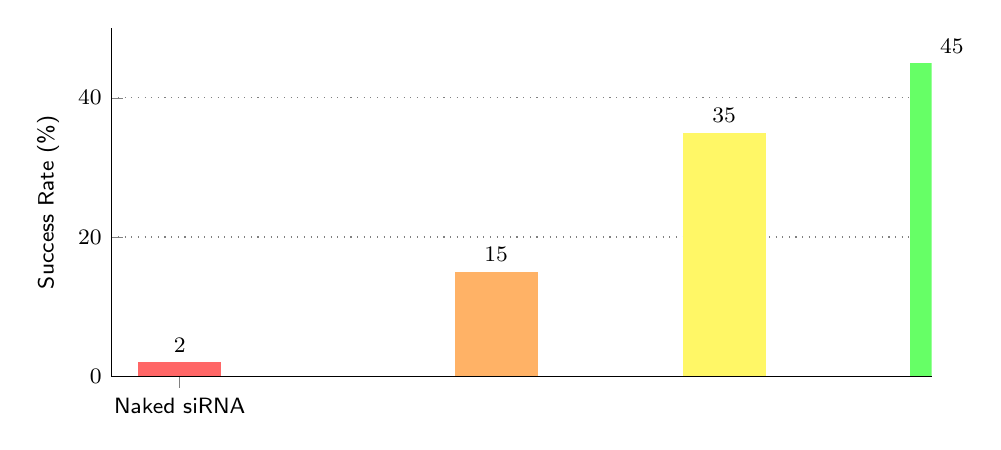
\begin{tikzpicture}
\begin{axis}[
    divergingstyle,
    ylabel={Success Rate (\%)},
    symbolic x coords={Naked siRNA, 1st Gen LNP, 2nd Gen LNP, GalNAc},
    xtick=data,
    xticklabel style={font=\footnotesize, text width=2.5cm, align=center},
    ymin=0, ymax=50,
]
\addplot[ybar, fill=red!60, draw=none] coordinates {(Naked siRNA, 2)};
\addplot[ybar, fill=orange!60, draw=none, forget plot] coordinates {(1st Gen LNP, 15)};
\addplot[ybar, fill=yellow!60, draw=none, forget plot] coordinates {(2nd Gen LNP, 35)};
\addplot[ybar, fill=green!60, draw=none, forget plot] coordinates {(GalNAc, 45)};
\end{axis}
\pgfplotsset{
    after end axis/.append code={
        \node[anchor=north, font=\tiny, text width=12cm, align=center] 
        at (current axis.south) [yshift=-1.5cm] {
            Note: Success rate defined as progression from Phase I to regulatory approval.\\
            Source: Industry Data, Morgan Stanley Research Analysis
        };
    }
}
\end{tikzpicture}
\end{center}

The evolution from naked siRNA (2\% success) to GalNAc conjugates (45\% success) represents a 20-fold improvement in clinical outcomes, directly correlating with commercial viability.

% --- SECTION 3: COMPETITIVE ANALYSIS ---
\section{Competitive Landscape \& Market Share}

\subsection{Market Share by Company (2025 Revenue)}

\begin{center}
\captionof{figure}{siRNA Therapeutics Market Share (2025, \$5.8B Total)}
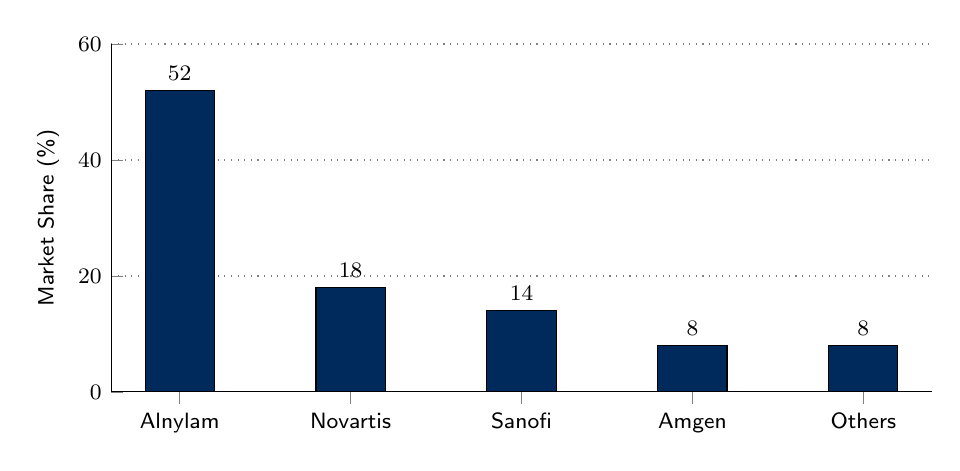
\begin{tikzpicture}
\begin{axis}[
    ybar,
    width=12cm,
    height=6cm,
    bar width=25pt,
    ylabel={Market Share (\%)},
    symbolic x coords={Alnylam, Novartis, Sanofi, Amgen, Others},
    xtick=data,
    xticklabel style={font=\footnotesize},
    yticklabel style={font=\footnotesize},
    ylabel style={font=\footnotesize},
    nodes near coords,
    nodes near coords style={font=\footnotesize\bfseries, color=black},
    ymin=0, ymax=60,
    ymajorgrids=true,
    grid style={dotted, gray},
    axis x line*=bottom,
    axis y line*=left,
]
\addplot[fill=msblue] coordinates {
    (Alnylam,52) (Novartis,18) (Sanofi,14) (Amgen,8) (Others,8)
};
\end{axis}
\pgfplotsset{
    after end axis/.append code={
        \node[anchor=north, font=\tiny, text width=12cm, align=center] 
        at (current axis.south) [yshift=-1.5cm] {
            Note: Market share based on 2025 estimated revenues. Novartis share includes Inclisiran royalties.\\
            Source: Company Filings, Morgan Stanley Research Estimates
        };
    }
}
\end{tikzpicture}
\end{center}

Alnylam maintains dominant market position with 52\% share, reflecting first-mover advantage \& comprehensive patent portfolio. However, increasing competition from major pharma partnerships suggests market share consolidation ahead.

\subsection{Competitive Positioning Matrix}

\begin{table}[H]
\centering
\caption{Key Players: Technology \& Market Position}
\label{tab:competitive_matrix}
\rowcolors{2}{msgrey}{white}
\tablefont
\begin{adjustbox}{max width=\textwidth}
\begin{tabular}{p{0.15\linewidth}p{0.18\linewidth}p{0.18\linewidth}p{0.15\linewidth}p{0.12\linewidth}p{0.15\linewidth}}
\toprule
\textbf{Company} & \textbf{Platform} & \textbf{Key Products} & \textbf{Pipeline} & \textbf{2025 Rev (\$M)} & \textbf{Growth Rate} \\
\midrule
Alnylam & GalNAc/LNP & Patisiran, Inclisiran & 45 programs & \$3,020 & 38\% \\
Novartis & Alnylam partnership & Inclisiran & 8 programs & \$1,045 & 55\% \\
Sanofi & In-licensed & Fitusiran & 12 programs & \$812 & 42\% \\
Amgen & Proprietary LNP & Olpasiran & 14 programs & \$465 & 28\% \\
Dicerna/Novo & GalXC & Nedosiran & 9 programs & \$458 & 35\% \\
\bottomrule
\end{tabular}
\end{adjustbox}
\par\vspace{0.1cm}
{\tiny Source: Company Reports, Morgan Stanley Research}
\end{table}

% --- SECTION 4: FINANCIAL PROJECTIONS ---
\section{Financial Analysis \& Valuation}

\subsection{Revenue Projection by Indication (2025-2030E)}

\begin{table}[H]
\centering
\caption{Market Size Forecast by Therapeutic Area (\$M)}
\label{tab:revenue_forecast}
\rowcolors{2}{msgrey}{white}
\tablefont
\begin{adjustbox}{max width=\textwidth}
\begin{tabular}{p{0.22\linewidth}p{0.12\linewidth}p{0.12\linewidth}p{0.12\linewidth}p{0.12\linewidth}p{0.12\linewidth}p{0.12\linewidth}}
\toprule
\textbf{Indication} & \textbf{2025} & \textbf{2026E} & \textbf{2027E} & \textbf{2028E} & \textbf{2029E} & \textbf{2030E} \\
\midrule
Rare Diseases & \$2,850 & \$3,420 & \$4,100 & \$4,920 & \$5,900 & \$7,080 \\
Cardiovascular & \$1,890 & \$2,650 & \$3,710 & \$5,190 & \$7,270 & \$10,180 \\
Metabolic & \$780 & \$1,090 & \$1,530 & \$2,140 & \$3,000 & \$4,200 \\
Oncology & \$280 & \$440 & \$690 & \$1,080 & \$1,690 & \$2,640 \\
\midrule
\textbf{Total} & \$5,800 & \$7,600 & \$10,030 & \$13,330 & \$17,860 & \$24,100 \\
\bottomrule
\end{tabular}
\end{adjustbox}
\par\vspace{0.1cm}
{\tiny Source: Morgan Stanley Research Estimates}
\end{table}

Note: Our revised 2030E forecast of \$24.1B represents significant upside to consensus of \$18B, driven by faster cardiovascular adoption \& oncology pipeline maturation.

\subsection{Growth Rate by Therapeutic Category}

\begin{center}
\captionof{figure}{CAGR by Therapeutic Area (2025-2030E)}
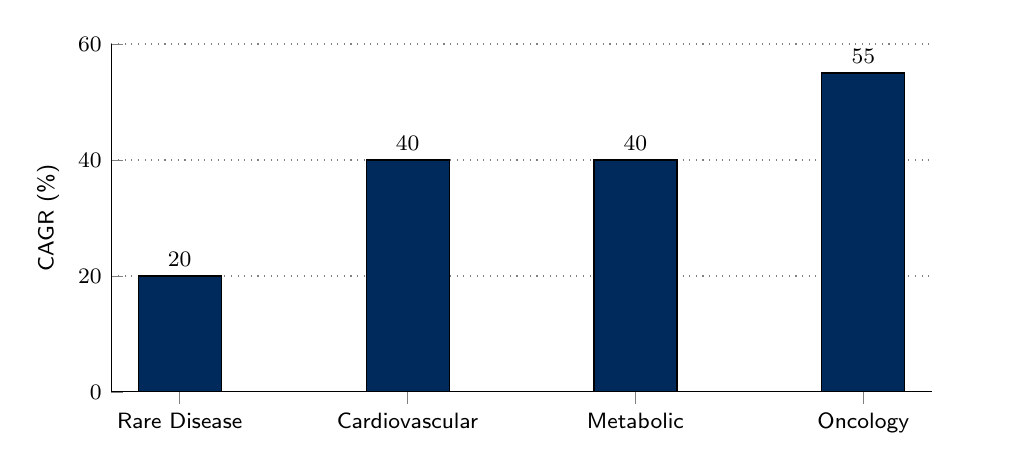
\begin{tikzpicture}
\begin{axis}[
    ybar,
    width=12cm,
    height=6cm,
    bar width=30pt,
    ylabel={CAGR (\%)},
    symbolic x coords={Rare Disease, Cardiovascular, Metabolic, Oncology},
    xtick=data,
    xticklabel style={font=\footnotesize, text width=3cm, align=center},
    yticklabel style={font=\footnotesize},
    ylabel style={font=\footnotesize},
    nodes near coords,
    nodes near coords style={font=\footnotesize\bfseries, color=black},
    ymin=0, ymax=60,
    ymajorgrids=true,
    grid style={dotted, gray},
    axis x line*=bottom,
    axis y line*=left,
]
\addplot[fill=msblue] coordinates {
    (Rare Disease,20) (Cardiovascular,40) (Metabolic,40) (Oncology,55)
};
\end{axis}
\pgfplotsset{
    after end axis/.append code={
        \node[anchor=north, font=\tiny, text width=12cm, align=center] 
        at (current axis.south) [yshift=-1.5cm] {
            Note: CAGR calculated from 2025 to 2030E. Oncology reflects Phase III readouts expected 2027-2028.\\
            Source: Morgan Stanley Research Estimates
        };
    }
}
\end{tikzpicture}
\end{center}

% --- SECTION 5: INVESTMENT RISKS ---
\section{Investment Risks \& Considerations}

\blueheader{Key Risk Factors}

While the siRNA market presents compelling growth opportunities, investors should consider several material risks:

\begin{table}[H]
\centering
\caption{Risk Assessment Matrix}
\label{tab:risk_matrix}
\rowcolors{2}{msgrey}{white}
\tablefont
\begin{adjustbox}{max width=\textwidth}
\begin{tabular}{p{0.22\linewidth}p{0.15\linewidth}p{0.15\linewidth}p{0.40\linewidth}}
\toprule
\textbf{Risk Category} & \textbf{Probability} & \textbf{Impact} & \textbf{Mitigation Strategy} \\
\midrule
Clinical Failure & Medium & High & Diversified pipeline across multiple MOAs \& targets \\
Manufacturing Scale-Up & Medium & Medium & Partnership with CDMOs; technology transfer programs \\
Regulatory Delays & Low & Medium & Early FDA engagement; orphan drug designations \\
Competition & High & Medium & Patent protection; first-mover advantage in key indications \\
Pricing Pressure & Medium & High & Value-based pricing; real-world evidence generation \\
Patent Expiry & Low & High & Next-generation platform development; indication expansion \\
\bottomrule
\end{tabular}
\end{adjustbox}
\par\vspace{0.1cm}
{\tiny Source: Morgan Stanley Research Analysis}
\end{table}

\subsection{Sensitivity Analysis: Market Size to Clinical Success Rate}

\begin{center}
\captionof{figure}{2030E Market Size Sensitivity (\$B)}
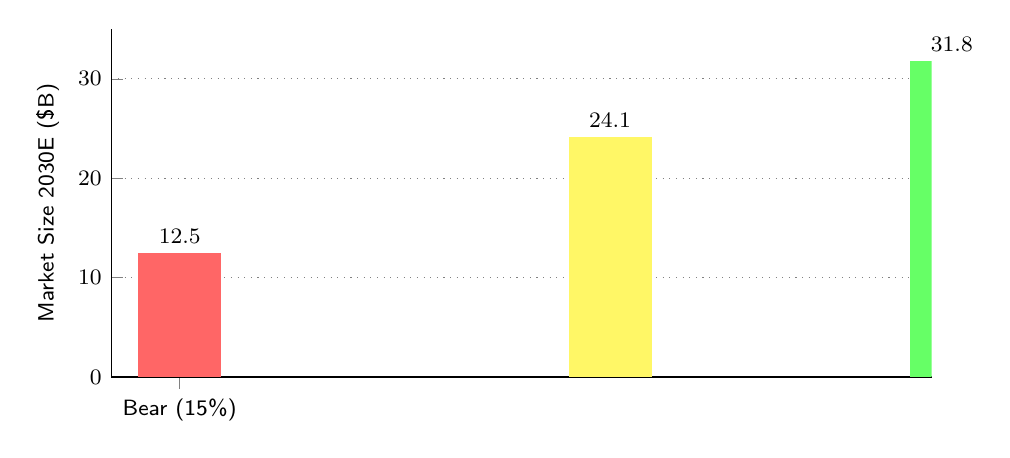
\begin{tikzpicture}
\begin{axis}[
    divergingstyle,
    width=12cm,
    ylabel={Market Size 2030E (\$B)},
    symbolic x coords={Bear (15\%), Base (22\%), Bull (30\%)},
    xtick=data,
    xticklabel style={font=\footnotesize, text width=3cm, align=center},
    ymin=0, ymax=35,
]
\addplot[ybar, fill=red!60, draw=none] coordinates {(Bear (15\%), 12.5)};
\addplot[ybar, fill=yellow!60, draw=none, forget plot] coordinates {(Base (22\%), 24.1)};
\addplot[ybar, fill=green!60, draw=none, forget plot] coordinates {(Bull (30\%), 31.8)};
\end{axis}
\pgfplotsset{
    after end axis/.append code={
        \node[anchor=north, font=\tiny, text width=12cm, align=center] 
        at (current axis.south) [yshift=-1.5cm] {
            Note: Scenarios based on Phase III success rates. Bear case assumes technology setbacks.\\
            Source: Morgan Stanley Research Sensitivity Analysis
        };
    }
}
\end{tikzpicture}
\end{center}

% --- SECTION 6: CONCLUSION ---
\section{Investment Conclusion \& Recommendations}

\insightbox{RATING: OVERWEIGHT}{
We rate the siRNA therapeutics sector OVERWEIGHT based on (1) accelerating clinical validation, (2) expanding addressable market beyond rare diseases, (3) improving delivery technology de-risking platforms, and (4) attractive risk/reward profile for diversified biotech portfolios.
}

\blueheader{Key Takeaways}

\begin{itemize}[leftmargin=*, itemsep=0.1cm]
    \item \textbf{Market Expansion:} Our \$24B 2030E forecast represents 33\% upside to consensus, driven by cardiovascular \& oncology pipeline maturation
    \item \textbf{Technology Validation:} 45\% Phase III success rate for GalNAc platforms significantly de-risks investment thesis
    \item \textbf{Competitive Dynamics:} Alnylam's dominance faces increasing challenge from big pharma partnerships, suggesting M\&A opportunities
    \item \textbf{Risk/Reward:} Current valuations (avg 8x 2027E sales) offer attractive entry point relative to historical biotech medians (12x)
\end{itemize}

\subsection{Top Picks \& Investment Strategy}

\begin{table}[H]
\centering
\caption{Recommended Investment Positions}
\label{tab:top_picks}
\rowcolors{2}{msgrey}{white}
\tablefont
\begin{adjustbox}{max width=\textwidth}
\begin{tabular}{p{0.18\linewidth}p{0.12\linewidth}p{0.18\linewidth}p{0.15\linewidth}p{0.15\linewidth}p{0.17\linewidth}}
\toprule
\textbf{Company} & \textbf{Ticker} & \textbf{Rating} & \textbf{Target Price} & \textbf{Upside} & \textbf{Key Catalyst} \\
\midrule
Alnylam Pharma & ALNY & Overweight & \$285 & 35\% & Cardiovascular expansion \\
Novartis & NVS & Equal-weight & \$118 & 15\% & Inclisiran ramp \\
Amgen & AMGN & Overweight & \$342 & 28\% & Olpasiran Phase III \\
Arrowhead Pharma & ARWR & Overweight & \$58 & 42\% & Platform validation \\
\bottomrule
\end{tabular}
\end{adjustbox}
\par\vspace{0.1cm}
{\tiny Source: Morgan Stanley Research. Target prices as of January 2026.}
\end{table}

\vspace{0.5cm}

\begin{center}
{\color{mstextgrey}\rule{0.8\textwidth}{0.5pt}}
\vspace{0.3cm}

{\footnotesize\bfseries Morgan Stanley Research}\\
{\footnotesize Healthcare Biotechnology Team}\\
{\footnotesize biotechnology@morganstanley.com}
\end{center}

\end{document}
